% PRIME Beamer Slides (English)
\documentclass{beamer}
\usetheme{Madrid}
\usecolortheme{default}

% Fonts & Encoding (keep it simple for portability)
\usepackage[utf8]{inputenc}
\usepackage{amsmath, amssymb}
\usepackage{graphicx}
\usepackage{hyperref}
\usepackage{booktabs}
\usepackage[table]{xcolor}

% Graphics path relative to slides/ (figures are under ../figures/images/)
\graphicspath{{../figures/images/}}

% Ensure table* works in beamer by mapping it to table
\newenvironment{table*}{\begin{table}}{\end{table}}

\title[PRIME]{PRIME: Process Reinforcement through Implicit Rewards}
\author{}
\institute{}
\date{\today}

\begin{document}

% Title
\begin{frame}
  \titlepage
\end{frame}

% Outline
\begin{frame}{Outline}
  \tableofcontents
\end{frame}

% =====================
% 1. Background
% =====================
\section{Background}

\begin{frame}{Motivation}
  \begin{itemize}
    \item RL for LLMs often uses outcome-only rewards (bandit setting): feedback only at the end of generation.
    \item Issues: reward sparsity, credit assignment, and vulnerability to spurious solutions.
    \item Dense process rewards can help but are hard to define, annotate, and update online at scale.
  \end{itemize}
\end{frame}

\begin{frame}{Key Challenges}
  \begin{itemize}
    \item C1: Process rewards are hard to define and expensive to annotate.
    \item C2: Online PRM updates are not scalable with step-level labels.
    \item C3: Dedicated reward modeling stage introduces extra data/compute costs.
  \end{itemize}
\end{frame}

\begin{frame}{High-level Illustration}
  \centering
  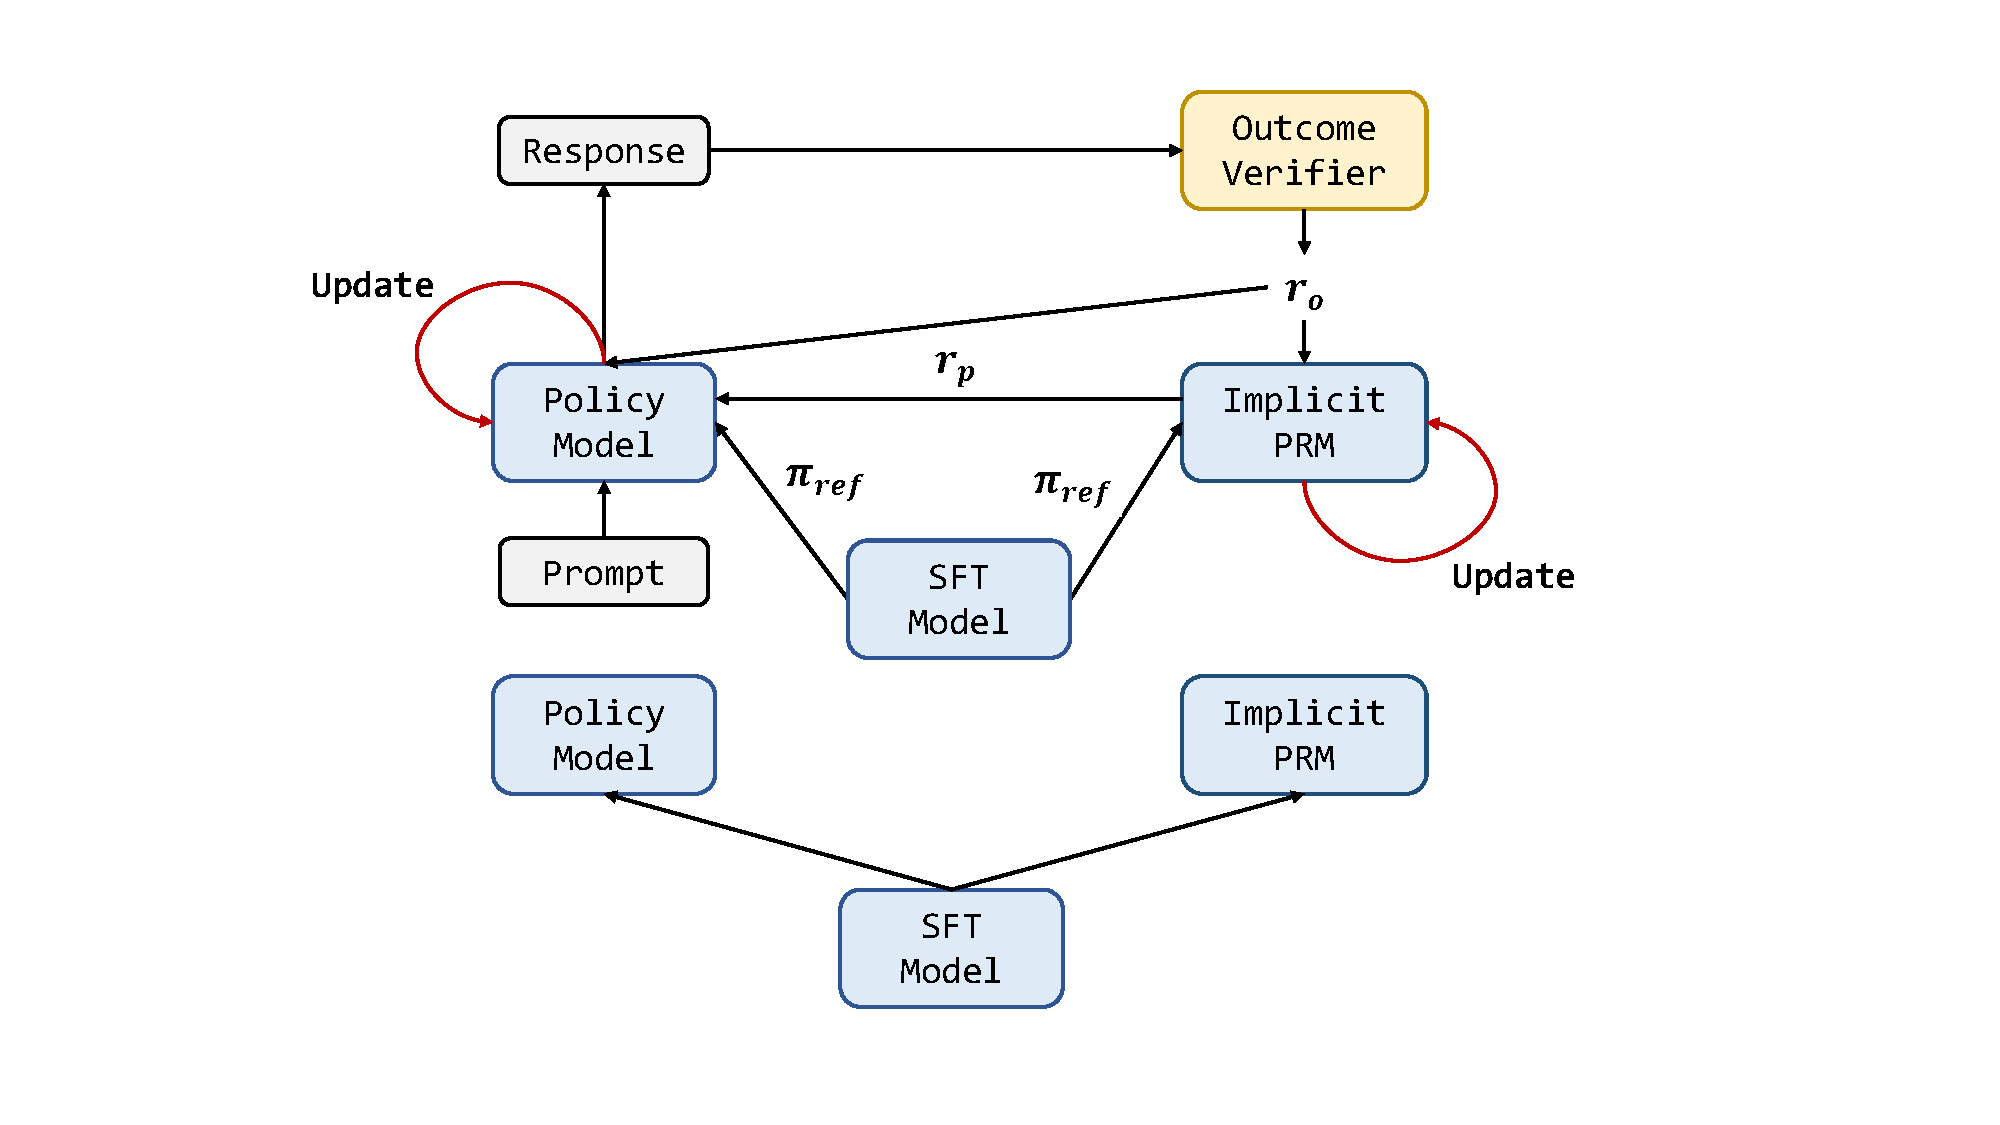
\includegraphics[width=0.9\linewidth]{prime-algo.pdf}\\[2mm]
  {\footnotesize PRIME leverages an Implicit PRM trained with outcome-only labels to yield token-level process rewards online.}
\end{frame}

% =====================
% 2. Algorithm
% =====================
\section{Algorithm}

\begin{frame}{Implicit Process Rewards (Core Idea)}
  \begin{itemize}
    \item Train an ``Implicit PRM'' with outcome-only labels:
    \[ r_\phi(\mathbf{y}) = \beta \log \frac{\pi_\phi(\mathbf{y})}{\pi_{\text{ref}}(\mathbf{y})} \]
    \item At inference, obtain token-level process rewards:
    \[ r_\phi(y_t) = \beta \log \frac{\pi_\phi(y_t\mid \mathbf{y}_{<t})}{\pi_{\text{ref}}(y_t\mid \mathbf{y}_{<t})} \]
    \item No step-level labels required; PRM can be updated online using policy rollouts and outcome labels.
  \end{itemize}
\end{frame}

\begin{frame}{Advantage Estimation (MC + RLOO)}
  \begin{itemize}
    \item Compute returns for process and outcome rewards separately, then sum as advantage.
  \end{itemize}
  \small
  \begin{align*}
  A^i_t =& \sum_{s=t}^{|\mathbf{y}^i|} \gamma^{s-t} \Big[r_\phi(y^i_s) - \tfrac{1}{K-1}\sum_{j\neq i} r_\phi(\mathbf{y}^j)\Big]\\
  &+ \Big[r_o(\mathbf{y}^i) - \tfrac{1}{K-1}\sum_{j\neq i} r_o(\mathbf{y}^j)\Big]
  \end{align*}
  \normalsize
  \vspace{2mm}
  \begin{itemize}
    \item Use PPO clip loss (or REINFORCE/GRPO/RLOO) for policy updates; PRIME is algorithm-agnostic.
  \end{itemize}
\end{frame}

\begin{frame}{PPO Clip Objective}
  \small
  \begin{align*}
    L_{\text{CLIP}}(\theta) = \mathbb{E}_t\Big[ \min\big(&\underbrace{\tfrac{\pi_\theta(y_t\mid \mathbf{y}_{<t})}{\pi_{\theta_{\text{old}}}(y_t\mid \mathbf{y}_{<t})}}_{\rho_t} A_t,\\
    &\text{clip}(\rho_t, 1-\epsilon, 1+\epsilon) A_t \big) \Big]
  \end{align*}
  \normalsize
  \vspace{1mm}
  {\footnotesize The clip prevents overly large policy updates and stabilizes training.}
\end{frame}

\begin{frame}{Training Loop (High-level)}
  \begin{enumerate}
    \item Initialize policy and PRM from the same SFT/base model; keep a reference model.
    \item Sample K responses per prompt; compute outcome rewards with a rule-based verifier.
    \item Online prompt filtering to stabilize difficulty distribution.
    \item Compute token-level process rewards via Implicit PRM; update PRM online with outcome labels.
    \item Build advantages (process + outcome, both with LOO) and update the policy (e.g., PPO clip).
  \end{enumerate}
\end{frame}

% =====================
% 3. Results Analysis
% =====================
\section{Results Analysis}

\begin{frame}{Performance and Efficiency}
  \begin{itemize}
    \item Significant gains on math and coding benchmarks starting from Qwen2.5-Math-7B-Base with light SFT.
    \item Higher sample efficiency than outcome-only RL (e.g., reaching same rewards in \~40\% steps).
    \item Per-step overhead \~24\%, but wall-clock efficiency \~2\texttimes{} due to faster convergence.
  \end{itemize}
\end{frame}

\begin{frame}{Training Curves}
  \centering
  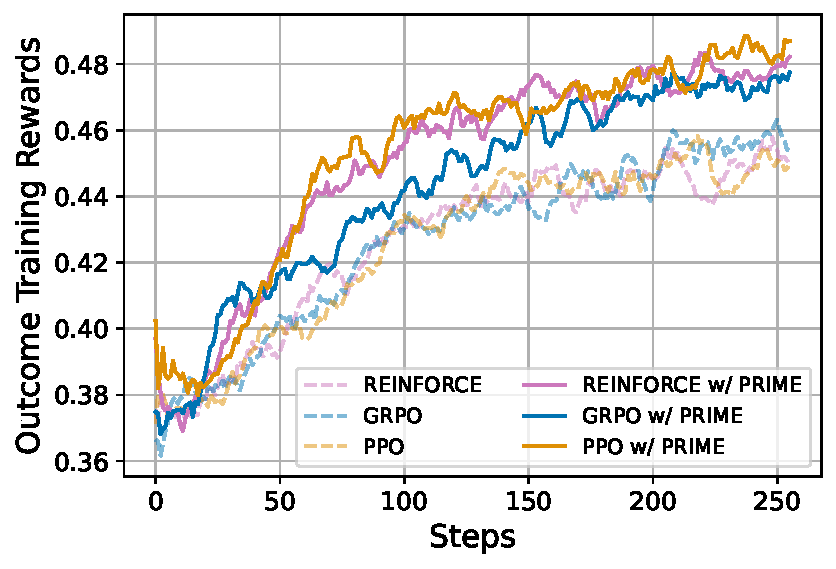
\includegraphics[width=0.9\linewidth]{train_rewards_baseline.pdf}\\[2mm]
  {\footnotesize PRIME generally improves stability and final rewards across RL baselines.}
\end{frame}

\begin{frame}{Overall Results}
  \centering
  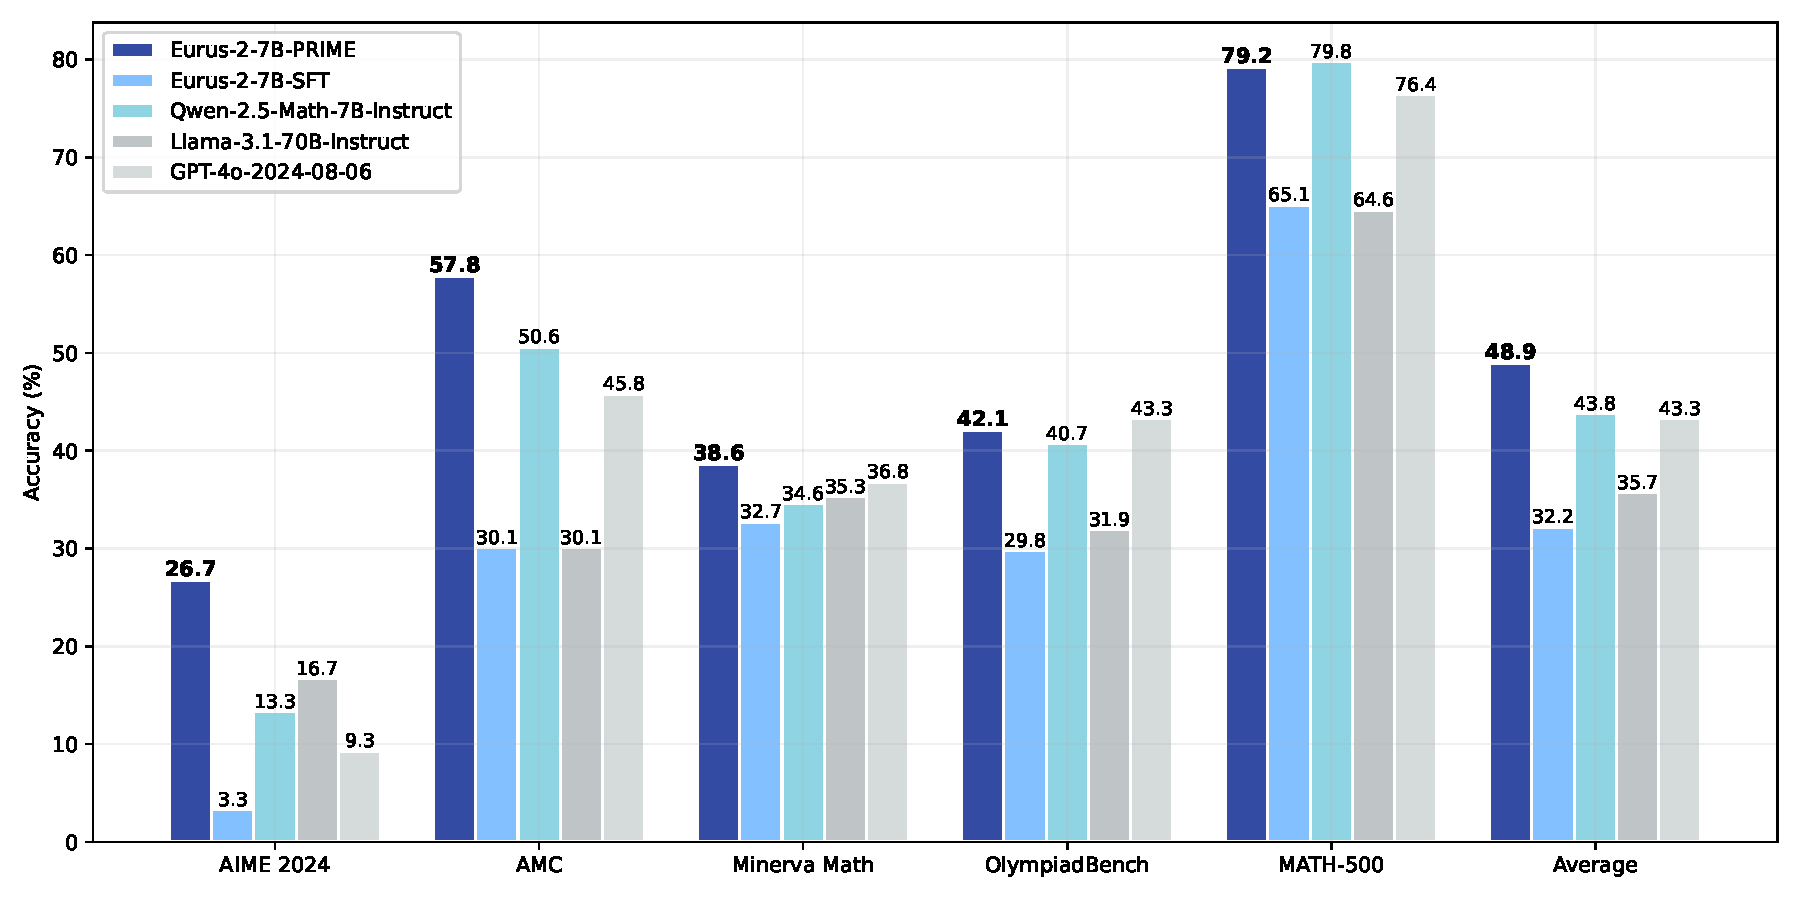
\includegraphics[width=0.9\linewidth]{results.pdf}\\[2mm]
  {\footnotesize Aggregate improvements on math/coding benchmarks.}
\end{frame}

\begin{frame}{Online PRM Matters}
  \centering
  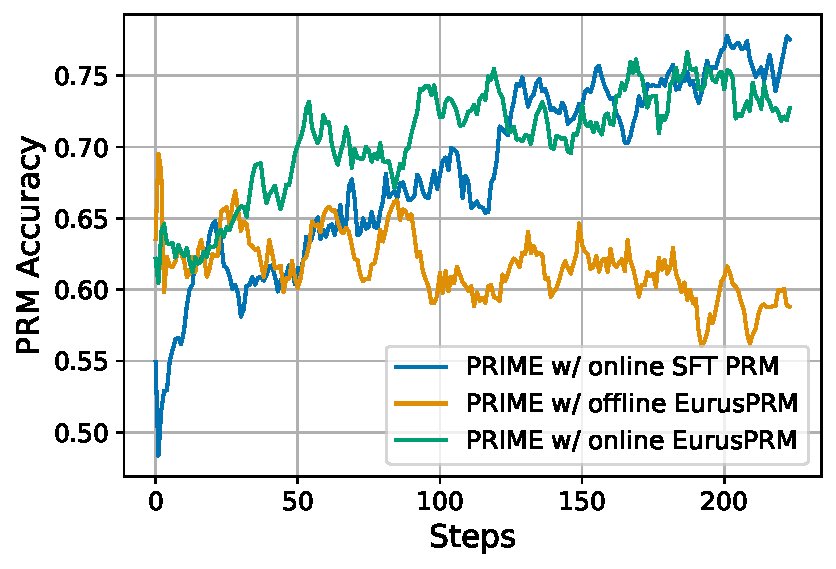
\includegraphics[width=0.9\linewidth]{prm_acc_online.pdf}\\[2mm]
  {\footnotesize Online updates maintain discrimination and avoid reward hacking as training progresses.}
\end{frame}

\begin{frame}{Ablation: Reference Choices}
  \centering
  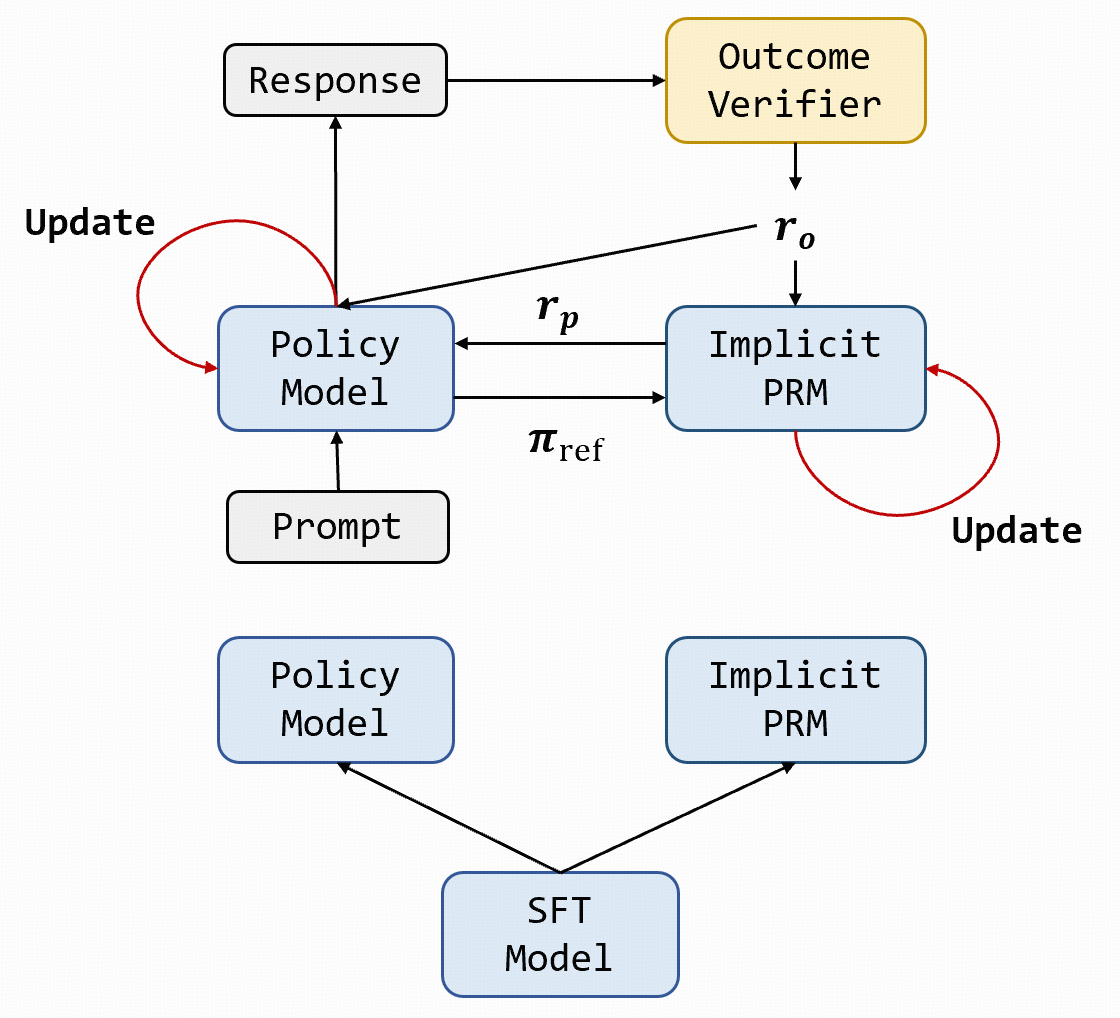
\includegraphics[width=0.48\linewidth]{policy_ref.png}\hfill
  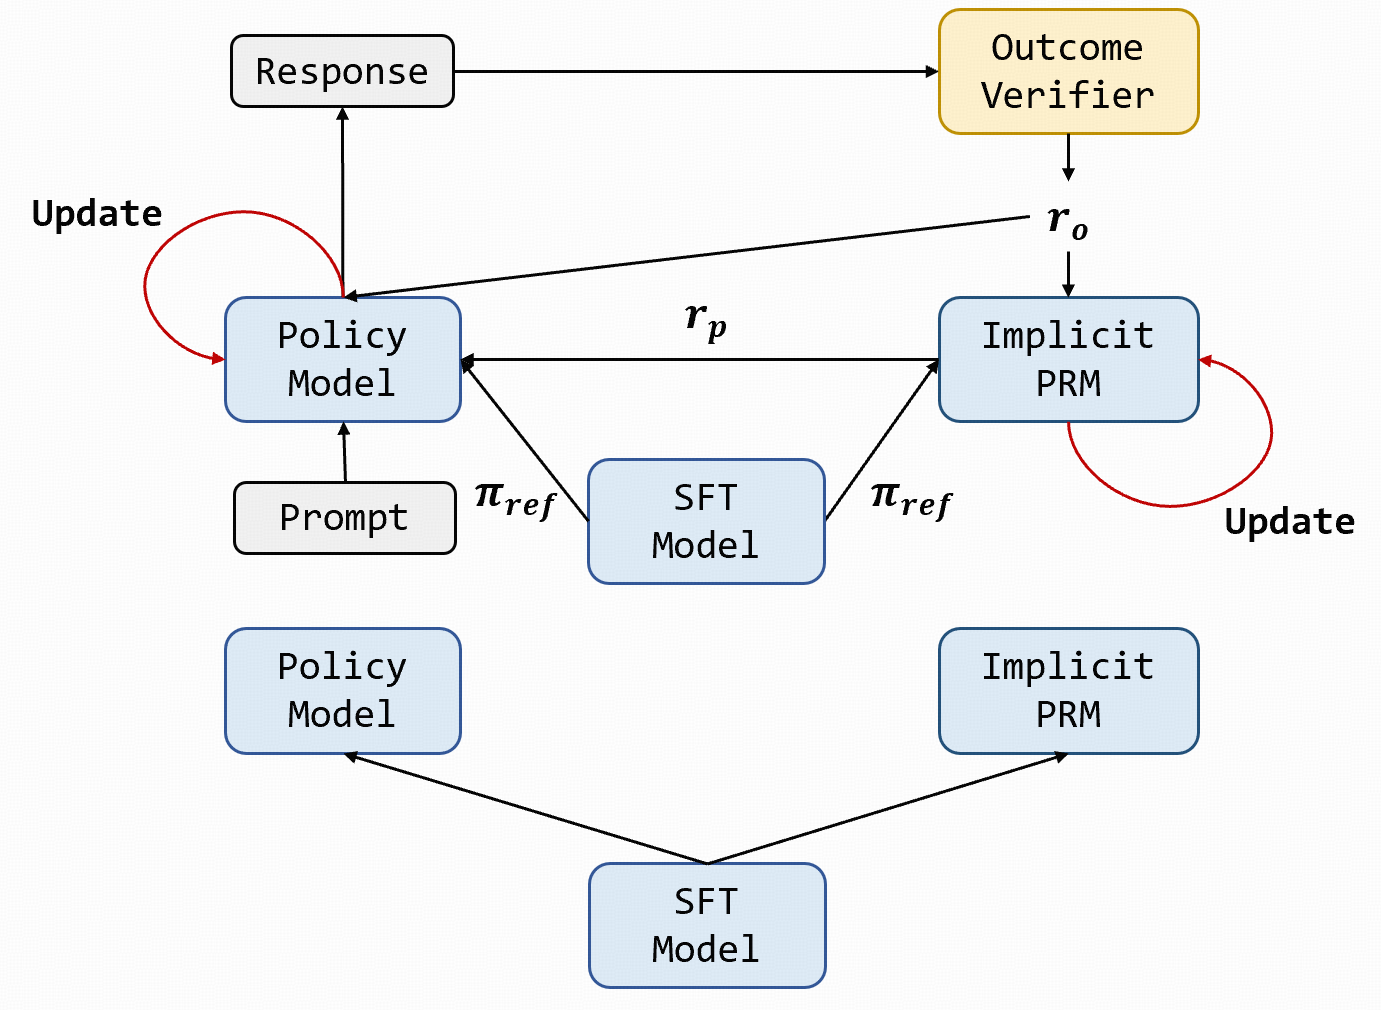
\includegraphics[width=0.48\linewidth]{sfr_ref.png}\\[2mm]
  {\footnotesize Using policy-old logits vs. a fixed SFT reference shows similar performance; each has pros/cons.}
\end{frame}

\begin{frame}{Table: Algorithms Comparison}
  \centering
  % Input a prebuilt table from the repository (uses booktabs and xcolor)
  \input{../tables/diff_rl_algo.tex}
\end{frame}

\begin{frame}{Ablations and Findings}
  \begin{itemize}
    \item PRM-as-reward \textgreater{} PRM-as-value or PPO value model: reward shaping works better than value baselines.
    \item SFT initialization for PRM \textgreater{} separately trained PRM: distribution alignment matters.
    \item Online PRM updates are key to avoid reward hacking and maintain discrimination between correct/wrong.
    \item PRIME benefits REINFORCE/GRPO/RLOO/PPO consistently; algorithm-agnostic plug-in.
  \end{itemize}
\end{frame}

% =====================
% 4. Limitations
% =====================
\section{Limitations}

\begin{frame}{Limitations}
  \begin{itemize}
    \item Model scale: experiments up to 32B; larger models and longer reasoning chains need further study.
    \item "Zero" RL (without SFT) can saturate early due to diversity drop; needs exploration mechanisms.
    \item Reference choice and single vs. double forward are engineering trade-offs depending on resources.
  \end{itemize}
\end{frame}

% Closing
\begin{frame}{Takeaways}
  \begin{itemize}
    \item PRIME enables scalable dense rewards for RL with LLMs via Implicit PRM trained with outcome labels only.
    \item Simple, efficient, and broadly compatible with common policy gradient methods.
  \end{itemize}
\end{frame}

\end{document}
